\chapter{Suggested solution}
\label{chp:suggested-solution}

In this chapter we'll walk through how the problem can be modelled and solved using linear programming.


\section{Modelling}

With some prior knowledge of graph algorithms, the first stab at solving the problem might be to look at our sample topologies and see a certain similarity to a max-flow problem -- edges have capacities, there's a set of sources, a set of sinks, and we want to maximize \emph{something}. However, there's a couple of things that make it hard to solve directly as a traditional flow problem, particularly that we don't have a single source and a single sink, but lots of them. Trying to model it as a single-source, single-sink problem quickly leads you to discover the limitations of that model, where you realize that if you actually solved, how would you be able to tell which node is generating flow on a given edge? Clearly, we need a way to distinguish node A's video from node B's video. And we need to make sure that all nodes receive video from every other node, not just maximum bitrate of \emph{any} video.

If we change perspective slightly, we see that this is not a single flow problem, but a \emph{series} of flow problems, sharing an underlying constrained resource. There's the problem of routing video from A to all other nodes, there's the problem of routing video from B to all other nodes, etc. In a conversation with $n$ participants, we now have $n$ separate flow problems, which all share the same resource. However, also this model is too limiting for our use case, as video is sent at a given bitrate, and this stream can neither be split at a given node without incurring a cost, nor does it make sense to add it; two 2Mbit videos cannot be joined to form a 4Mbit video. If you put enough restrictions on your nodes and edges it's probable that you might be able to able to prevent this from happening, but there's another way.\todo{Insert graph showing how this fails. Does it fail it any obvious way? With flow conservation on the nodes it doesn't seem like it, actually. But it might be harder to add restrictions on re-encoding later. Or it's a completely valid option, open for further investigation.}

This time around, imagine that we have a separate flow problem for each \emph{pair} of nodes; we have one problem routing node A's video to node B, we have one problem routing node A's video to node C, etc. This yields a total of $n(n-1)$ problems, which is $O(n^2)$. Modelling the problem this way means we don't have to add any supernodes to connect the targets, each node can act as sink for its own video stream, hereafter known as the \emph{commodity}, destined for itself.

One other thing we notice from our initial graph compared to traditional flow problems is that we notice that we have \emph{node constraints} in the initial graph, while flow problems only work on \emph{edge constraints}. To accommodate this, we split each node into two parts, hereafter called the external and internal part, as illustrated in \autoref{fig:node-splitting}.

\begin{figure}
    \centering
    \begin{subfigure}[t]{.48\textwidth}
        \centering
        \includegraphics[width=\textwidth]{nodesplitting-pre}
        \subcaption{Original problem}
    \end{subfigure}
    \hfill
    \begin{subfigure}[t]{.48\textwidth}
        \centering
        \includegraphics[width=\textwidth]{nodesplitting-post}
        \subcaption{Problem after node splitting}
    \end{subfigure}
    \caption{How node splitting works}
    \label{fig:node-splitting}
\end{figure}

As we now have a well-specified way to go from a given conversation to a graph that can be solved by max-flow algorithms, the entire problem can be solved by joining all the different subproblems under the same resource constraints, and solve as a multi-commodity max-flow problem. This class of problems can be solved with linear programming, which can be summarized in canonical form as \todo{Insert LP formulation here}.

As LP is a well-known and very general technique that's effective to a vast collection of problems, there are lots of LP-solvers freely available\footnote{\url{https://en.wikipedia.org/wiki/Linear_programming#Solvers_and_scripting_.28programming.29_languages}}. This simplifies building a solution on top of LP, if you can model your problem as a linear program, it can be efficiently solved by well-tested code. For our experimental solution the GNU Linear Programming Kit (GLPK) was chosen somewhat arbitrarily, as it has Python-bindings provided by the \texttt{glpk}\footnote{\url{https://pypi.python.org/pypi/glpk}}-package.


\section{Maximization}

Then there's the issue of the \emph{something} we wanted to maximize in the problem. If you want to consider the full picture with users influenced by mood, context and lots of other human factors that come into play, this is a complex topic that could warrant several papers on its own. In this thesis we'll simplify the problem to only consider two factors that influence our decision: bandwidth and latency. Thus, our reformulated problem is to \emph{maximize} bandwidth of each commodity at a \emph{minimal} latency. Formulated for each node in a conversation, this becomes our \emph{objective function}. The weighting between the two can be parametrized and left for implementations to decide.

In any case, this raises some other issues that has to be handled. The objective function has to be linear to be solved as a linear program, but several of our parameters are non-linear. Perceived gain from increasing bandwidth is non-linear, the cost of link utilization is non-linear, and perceived gain from reducing latency is probably non-linear. However, all of these can be approximated arbitrarily close by a piecewise linear function, as illustrated in \todo{Insert example of piecewise linear functions}. This too can be parametrized, as either the number of pieces to divide into or as the maximum deviation from the true allowed.

These different cases will be discussed in the following paragraphs, before we arrive at our final objective function.


\section{Perceived Gain From Bandwidth}

Increasing the bitrate of video is subject to diminishing returns, increasing the bitrate from 1Mbps to 2Mpbs yields a bigger return for the user than going from 4Mbps to 5Mbps. x264, the H.264 encoder powering applications like VLC\footnote{\url{http://www.videolan.org/developers/x264.html}}, HandBrake\footnote{\url{https://handbrake.fr/}} and ffmpeg\footnote{\url{https://trac.ffmpeg.org/wiki/Encode/H.264}}, uses an exponential scale for the relationship between bitrate and perceived quality\footnote{\url{https://trac.ffmpeg.org/wiki/Encode/H.264#crf}}, as illustrated in \autoref{fig:bitrate-quality}.

\begin{figure}
    \centering

    \begin{tikzpicture}
        \begin{axis}[
            xlabel=Quality,
            ylabel=Bitrate,
            xmin=0,
            ymin=0
        ]

        \addplot+[domain=0:51]{e^{-x}};
        \label{fig:utility-latency}
        \end{axis}
    \end{tikzpicture}

    \caption{The relationship between bitrate and quality in the x264 project}
    \label{fig:bitrate-quality}
\end{figure}


\section{Link Utilization}

The cost of utilizing a given network link is a function of the link's utilization, which is given by the classic queuing delay formula, $1/(1 - \mu/\lambda)$. As can be seen in \autoref{fig:utility-latency}, this function is not linear, and can thus not be used directly in our objective function. Nonetheless, we can achieve the same goal -- punishing over-utilization of individual links -- by approximating the function with a piecewise linear graph. The following algorithm partitions a set of slots into a set of edges:

\todo{Insert partitioning-algo here}

Based on this formula, we can formulate the cost multiplier of a link as $1 + k/(\mu - \lambda)$, where $k$ is a customizable parameter for how heavily link saturation should be punished. In our experiments, $k=10$ seems appropriate. This cost function can be seen in \autoref{fig:utility-latency}. We then partion this function into a small set of piecewise linear intervals, which we can model as parallell edges between two nodes, with different capacities and costs. Keeping this set small limits the number of variables in the resulting matrix, and thus keeps processing times reasonably low.

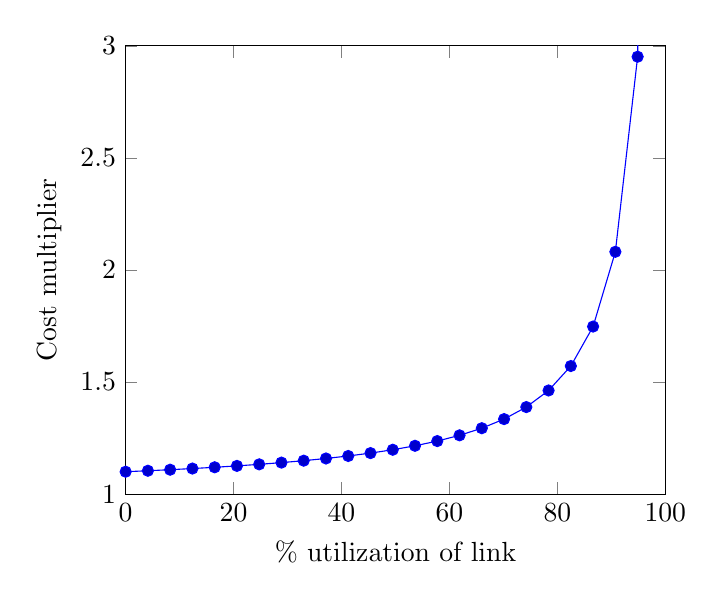
\begin{tikzpicture}
    \begin{axis}[
        xlabel={\% utilization of link},
        ylabel={Cost multiplier},
        xmin=0,
        ymin=1,
        ymax=3,
        xmax=100]

    \addplot+[domain=0:99]{1 + 10/(100 - x)};
    \label{fig:utility-latency}
    \end{axis}
\end{tikzpicture}


\begin{center}
    \label{tab:utilization-to-cost}
    \begin{tabular}{| l | l |}
    \hline
    \textbf{Link utilization} & \textbf{Cost multiplier} \\ \hline
    0--50\% & 1.2 \\ \hline
    51--75\% & 1.40 \\ \hline
    76--80\% & 1.50 \\ \hline
    81--90\% & 2.00 \\ \hline
    \end{tabular}
\end{center}

Using this partitioning as a guide, we can map any number of slots on a physical link into a set of edges $E$ in our graph where $|E| <= 4$.




\subsection{Alternative model}

One alternative way to model the problem, is to skip the node splitting step of the previous model, and instead connect nodes directly, but stay below bandwidth by adding constraints for the total sum going out from each node. Which model to choose is -- as in every engineering matter -- a question of priorities. The first model is a bit harder to comprehend initially, but results in fewer total edges than the latter model does when $n>3$, as can be seen in \autoref{fig:model-scaling}. Edge counts do not matter that much when $n$ is low as finding a solution will occur in trivial time anyway, but the difference might be substantial when n is larger. \todo{If performance ends up being an issue for larger graphs, add a note here about more research being needed into optimizing performance, as alternative models might be an avenue to explore for achieving that.}

\begin{figure}
\centering
    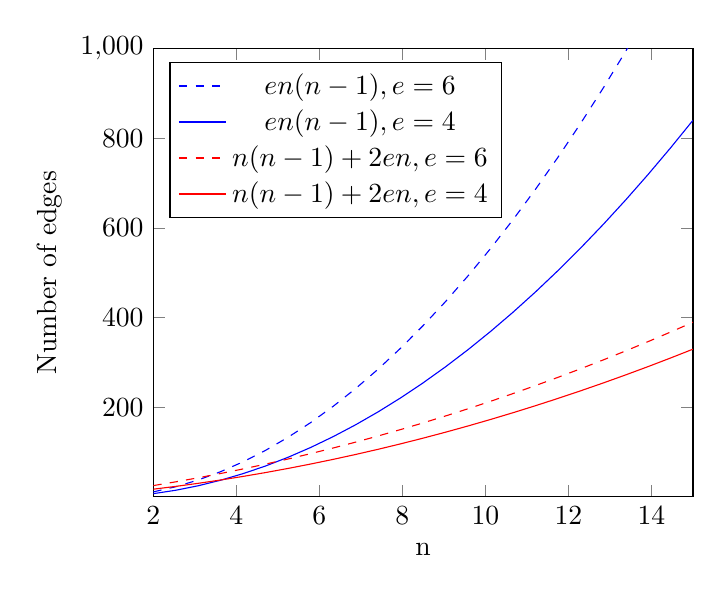
\begin{tikzpicture}
        \begin{axis}[
            xlabel={n},
            ylabel={Number of edges},
            xlabel near ticks,
            ylabel near ticks,
            legend pos=north west,
            xmin=2,
            ymin=1,
            ymax=1000,
            xmax=15]

        \addplot+[dashed, domain=2:15, mark=none, color=blue]{6*x*(x-1)};
        \addlegendentry{$en(n-1), e=6$}

        \addplot+[domain=2:15, mark=none, color=blue]{4*x*(x-1)};
        \addlegendentry{$en(n-1), e=4$}

        \addplot+[dashed, domain=2:15, mark=none, color=red]{x*(x-1) + 2*x*6};
        \addlegendentry{$n(n-1) + 2en, e=6$ }

        \addplot+[domain=2:15, mark=none, color=red]{x*(x-1) + 2*x*4};
        \addlegendentry{$n(n-1) + 2en, e=4$ }
        \label{fig:utility-latency}
        \end{axis}
    \end{tikzpicture}
    \caption{How the number of edges in the graph scales for different modeling techniques.}
    \label{fig:model-scaling}
\end{figure}


\section{The Algorithm}

Given the model, how do you efficiently find the "best" topology?


\section{Implementation}\label{sec:implementation}

\todo{Write about how the implementation was done}


\section{Tuning}

How can the algorithm be tuned, and how was the parameters chosen?
